\documentclass[10pt, compress]{beamer}

% \usetheme{m}
\usepackage[normalem]{ulem}
\usepackage{booktabs}
\usepackage[scale=2]{ccicons}
\usepackage{minted}

\usepackage{tikz}
\usepackage{gantt}
          
\usepackage{tikz}
\usemintedstyle{trac}

\title{Joint Causal Inference (JCI) and protein signalling networks}
\subtitle{Applying the JCI framework to real-world data}
\date{\today}
\author{Alex Khawalid\\\textbf{Supervisor:} Sara Magliacane}
\institute{Universiteit van Amsterdam}

\begin{document}

\maketitle

% \begin{frame}
%     \frametitle{Introduction}
%     The following topics will be discussed
%     \begin{itemize}
%         \item What is JCI?
%         \item What will be researched in this thesis?
%         \item What method will be used?
%         \item What kind of schedule can be expected?
%     \end{itemize}
% \end{frame}

\begin{frame}
    \frametitle{Introduction}
    % \textbf{Preliminary knowledge to understand the problem}
    \begin{itemize}
        \item \textit{Causal Discovery:} \begin{itemize}
            \item a field in statistics
            \item aims to uncover causal relations
        \end{itemize}
        \item \textit{Causal relations:}\begin{itemize}
            \item given an intervention that changes a variable X, if a variable Y changes then X causes Y
            \item can be represented by causal graphs
        \end{itemize}
        \item \textit{Joint Causal Inference (JCI):} \begin{itemize}
            \item a framework to do causal discovery over multiple datasets
            \item requires specific algorithms because of deterministic relations
            \item do not scale well, can only handle 6 variables % not sufficient for real datasets
        \end{itemize}
        \item Non-deterministic JCI \begin{itemize}
            \item simplified version, no deterministic relations
            \item no implementation yet
            \item expected to scale better, so can be applied to real world data
        \end{itemize}
    \end{itemize}
\end{frame}

% \begin{frame}{What is Non-deterministic JCI?} 
    
%   \begin{figure}
%     \centering
%     \includegraphics[width=\textwidth]{assignment4_cmap.png}
%     \caption{An overview of how JCI fits into the bigger picture}
%   \end{figure}
% \end{frame}

\section{Research question}
\begin{frame}
    \frametitle{Research question}
    \begin{itemize}
        \item \textbf{Main goal of thesis:}
            \begin{itemize}[<+- | alert@+>]
                \item How does JCI perform on a real-world dataset,  e.g. protein signaling network? 
            \end{itemize}
    
        \item\textbf{The problem:}
            \begin{itemize}[<+- | alert@+>]
                \item JCI cannot scale to the required number of variables
            \end{itemize}
    
        \item\textbf{Solution:}
            \begin{itemize}[<+- | alert@+>]
                \item Implement an algorithm for non-deterministic JCI
                \item Add intervention variables to the data that are not determinstically related
            \end{itemize}
    \end{itemize}
\end{frame}

% gfci vs fges
% gfci constraint
% fges score-based, pattern of graphs with small balls instead of arrows

\section{Approach}
\begin{frame}
    \frametitle{Approach}
    \textbf{How can we implement non-deterministic JCI?}
    \bigskip
    
    
    \textbf{Proposed method:}
    \begin{itemize}
        \item Find Deterministic relations
        \item Remove deterministic relations
        \item Add forbidden edges from system variables to intervention variables
        \item Apply GFCI to non-deterministic JCI
        \item Test on data real world
    \end{itemize}

\end{frame}


\section{Results}
\begin{frame}
    \frametitle{Results}
    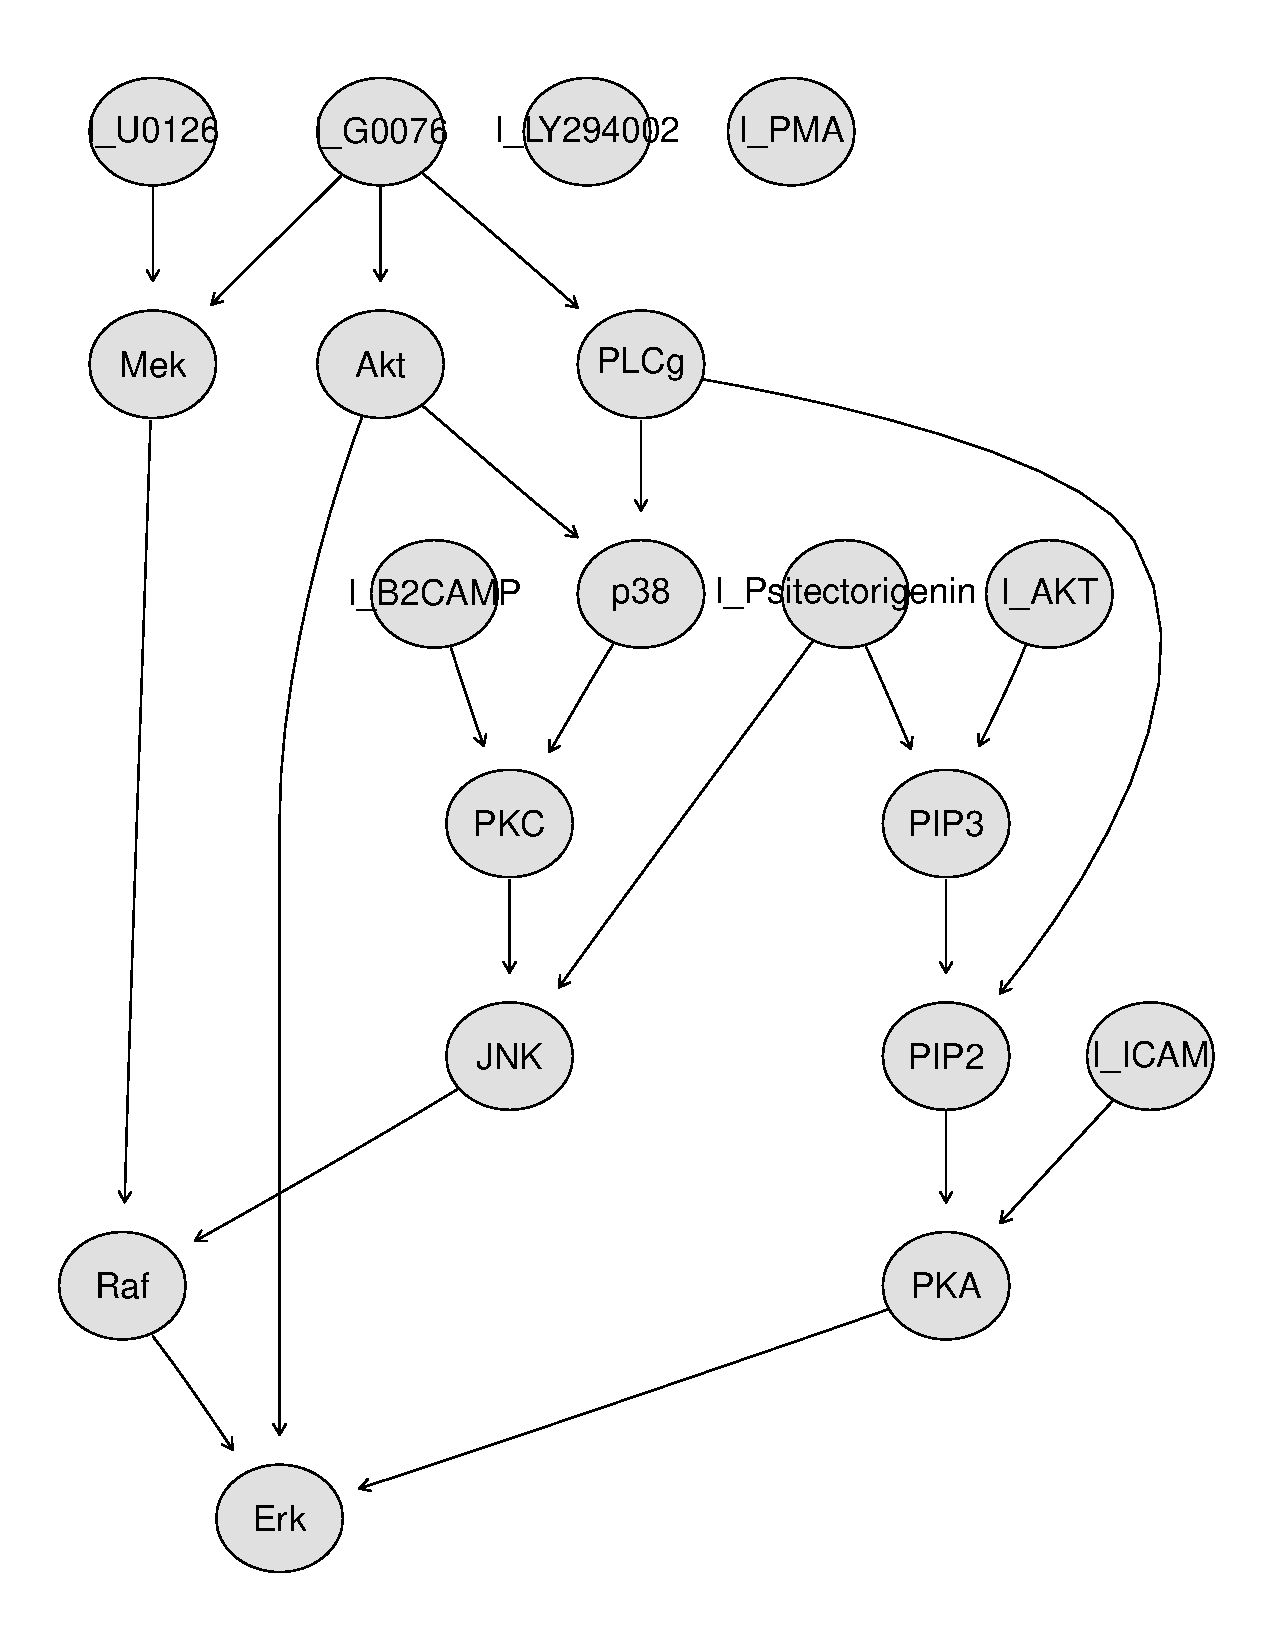
\includegraphics[width=0.5\textwidth]{gfci_plot}%
    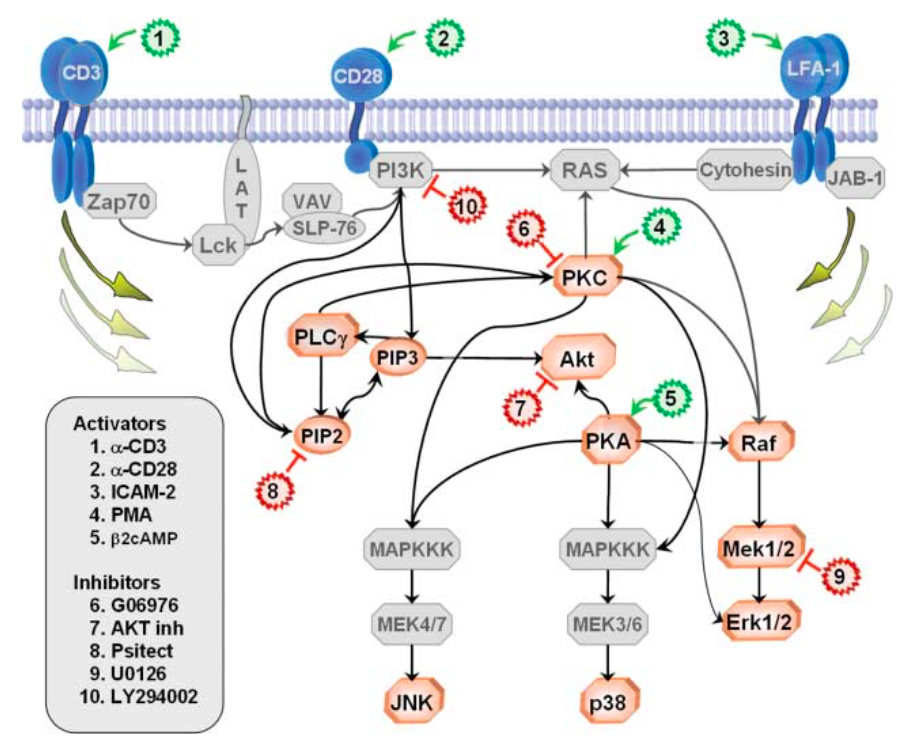
\includegraphics[width=0.5\textwidth]{sachs_plot}
    % add sachs graph
    % add gfci graph
\end{frame}

% detailed background: no hidden variables that cause both intervention variables and system variables
\section{Plan}
\begin{frame}
    \frametitle{Schedule}
    \textbf{Milestones}
    \begin{itemize}
        \item \sout{find and remove deterministic relations}
        \item\sout{add forbidden edges}
        \item \sout{first application to data}
        \item add more detailed background knowledge
        \item explore different parameters with simulated data
        \item improve results on real data
    \end{itemize}
    
\end{frame}

\begin{frame}
\frametitle{Schedule}
    \begin{figure}
        \centering
        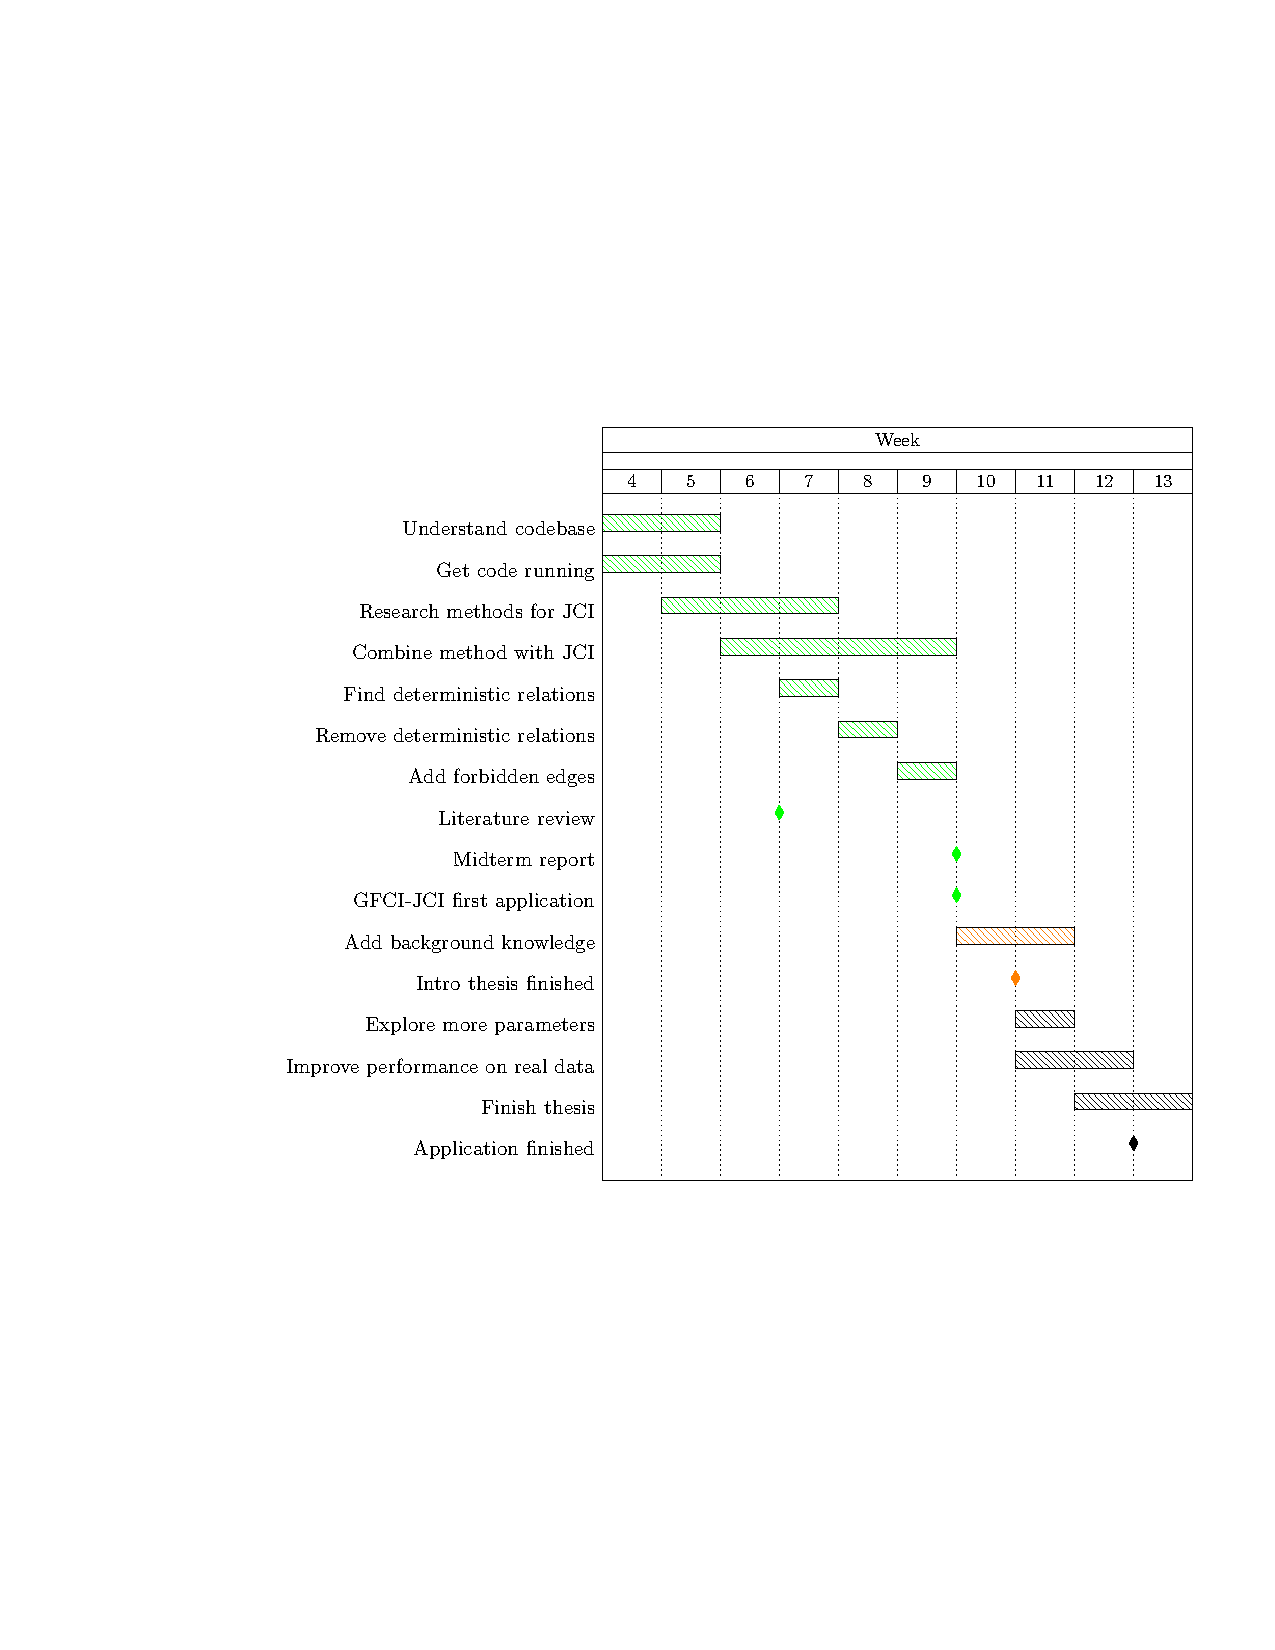
\includegraphics[width=\textwidth]{gantt.pdf}
        \caption{Caption}
        \label{fig:my_label}
    \end{figure}
\end{frame}

\section{Questions}
\begin{frame}{}
\begin{center}
\Huge \textbf{Questions?}
\end{center}
\end{frame}

\end{document}
